\documentclass[pdflatex,compress]{beamer}

\usetheme[darktitle,framenumber,totalframenumber]{UniversiteitAntwerpen}
%\usetheme[light,framenumber,totalframenumber]{UniversiteitAntwerpen}

\usefonttheme[onlymath]{serif}
\usepackage{lipsum}
\setbeamertemplate{caption}[numbered]
\beamertemplatenavigationsymbolsempty

\usepackage[
backend=biber,
style=authoryear,
]{biblatex}
\addbibresource{bibliography.bib}

% For advanced caption options, especially making some captions smaller
\usepackage{caption}

% For bold math characters
\usepackage{bm}

% For math stuff, e.g. align
\usepackage{amsmath}

% For quotations
\usepackage{csquotes}

% To make \parencite use brackets instead of braces
\DeclareCiteCommand{\parencite}
  {\usebibmacro{prenote}}
  {\usebibmacro{citeindex}%
   \printtext[bibhyperref]{[\usebibmacro{cite}]}}
  {\multicitedelim}
  {\usebibmacro{postnote}}

\title{Learning and Memorization}
%\subtitle{This is a dummy subti}

\author{Bernhard Gstrein}

\begin{document}

\maketitle

\AtBeginSection[]{}

\begin{frame}
\frametitle{Motivation}
\begin{itemize}
	\item \parencite{zhang2017understanding}: neural networks have the capacity to memorize their training set 
		\begin{itemize}
			\item Train AlexNet on CIFAR-10 with randomly permuted labels
			\item Training error goes to 0
		\end{itemize}
		\vspace{1em}
	\item What is the link between \textbf{memorization} and \textbf{generalization}?
		\begin{itemize}
		\item Why don't NNs just memorize their training set?
		\end{itemize}
		\vspace{1em}
	\item \parencite{chatterjee2018learning}: Is it possible to generalize by memorizing alone?
\end{itemize}
\end{frame}

\begin{frame}
	\frametitle{Basic idea of paper}
		\begin{itemize}
			\item What is a simple form of memorization? $\rightarrow$ a table
		\end{itemize}
		\vspace{1em}
		\small
		\begin{minipage}{.95\linewidth}\centering
			\begin{minipage}[b]{.6\linewidth}
			\begin{table}[]
			\begin{tabular}{ccc}
			Lives in water          & Has eyes               & Has limbs              \\ \hline
			\multicolumn{1}{|c|}{0} & \multicolumn{1}{c|}{1} & \multicolumn{1}{c|}{1} \\ \hline
			\multicolumn{1}{|c|}{1} & \multicolumn{1}{c|}{1} & \multicolumn{1}{c|}{0} \\ \hline
			\multicolumn{1}{|c|}{1} & \multicolumn{1}{c|}{0} & \multicolumn{1}{c|}{0} \\ \hline
			\end{tabular}
			\end{table}
		\end{minipage}
		\begin{minipage}[b]{.2\linewidth}
				\begin{table}[]
				\begin{tabular}{c}
				Vertebrate              \\ \hline
				\multicolumn{1}{|c|}{1} \\ \hline
				\multicolumn{1}{|c|}{1} \\ \hline
				\multicolumn{1}{|c|}{0} \\ \hline
				\end{tabular}
				\end{table}
			\end{minipage}
		\end{minipage}
	\centering
	Model for classification of animals into vertebrates/invertebrates
	\normalfont
	\vspace{1em}
	\begin{itemize}
		\item We must binarize the dataset
		\item We must limit the complexity
			\begin{itemize}
				\item 28x28 images \, $\rightarrow$ \, $28 \cdot 28 = 784$ \, $\rightarrow$ \, $2^{784} \propto 10^{236}$
			\end{itemize}
	\end{itemize}
\end{frame}

\AtBeginSection[]
{
  \begin{frame}
    \frametitle{Table of Contents}
    \tableofcontents[currentsection]
  \end{frame}
}

\section{Single lookup table ("lut")}

\begin{frame}
	\frametitle{Preprocessing data}
	\begin{itemize}
		\item MNIST dataset: 28x28 images of handwritten digits (0-9)
		\item We unroll the images: $28 \cdot 28 = 784$
		\item We scale the numerical values to the range $[0,1]$
		\item We binarize the data using the operator $>0.5$
		\item Labels (to be predicted): class 0-4 vs. 5-9
	\end{itemize}
	\vspace{1em}
	\begin{itemize}
		\item We end up with
			\begin{itemize}
				\item Features: matrix of shape $(N, 784)$, boolean entries
				\item Labels: matrix of shape $(N, 1)$, boolean entries
			\end{itemize}
	\end{itemize}
\end{frame}

\begin{frame}
	\frametitle{A single lut}
	\begin{itemize}
		\item Reminder: every example is an instance of a \enquote{bit pattern} (e.g. $\bm{x}^i=010$) and has a label (e.g. $y^i=1$)
		\item For each bit pattern, we cound how many times $y=0$ and $y=1$
	\end{itemize}
	\begin{align*}
		\hat{f}(\text{bit pattern}) =
		\begin{cases}
			0 & \text{if} \hspace{1em} \sum\limits_{y=0} > \sum\limits_{y=1} \\
			1 & \text{if} \hspace{1em} \sum\limits_{y=0} < \sum\limits_{y=1} \\
			\text{rand}(0,1) & \text{if} \hspace{1em} \sum\limits_{y=0} = \sum\limits_{y=1}
		\end{cases}
	\end{align*}
\end{frame}

\begin{frame}
	\frametitle{A single lut: example}
	\small
		\begin{minipage}{.95\linewidth}\centering
			\begin{minipage}[b]{.2\linewidth}\centering
				\begin{align*}
					\begin{array}{cc}
						\bm{x}                         & y                      \\ \hline
						\multicolumn{1}{|c|}{000} & \multicolumn{1}{c|}{0} \\ \hline
						\multicolumn{1}{|c|}{000} & \multicolumn{1}{c|}{1} \\ \hline
						\multicolumn{1}{|c|}{000} & \multicolumn{1}{c|}{1} \\ \hline
						\multicolumn{1}{|c|}{001} & \multicolumn{1}{c|}{1} \\ \hline
						\multicolumn{1}{|c|}{100} & \multicolumn{1}{c|}{0} \\ \hline
						\multicolumn{1}{|c|}{110} & \multicolumn{1}{c|}{0} \\ \hline
						\multicolumn{1}{|c|}{110} & \multicolumn{1}{c|}{1} \\ \hline
					\end{array}
				\end{align*}
			\end{minipage}
			\begin{minipage}[b]{.4\linewidth}\centering
				\begin{align*}
					\begin{array}{ccc}
						\text{bit pattern}        & \sum\limits_{y=0}      & \multicolumn{1}{l}{\sum\limits_{y=1}} \\ \hline
						\multicolumn{1}{|c|}{000} & \multicolumn{1}{c|}{1} & \multicolumn{1}{c|}{2}                \\ \hline
						\multicolumn{1}{|c|}{001} & \multicolumn{1}{c|}{0} & \multicolumn{1}{c|}{1}                \\ \hline
						\multicolumn{1}{|c|}{010} & \multicolumn{1}{c|}{0} & \multicolumn{1}{c|}{0}                \\ \hline
						\multicolumn{1}{|c|}{011} & \multicolumn{1}{c|}{0} & \multicolumn{1}{c|}{0}                \\ \hline
						\multicolumn{1}{|c|}{100} & \multicolumn{1}{c|}{1} & \multicolumn{1}{c|}{0}                \\ \hline
						\multicolumn{1}{|c|}{101} & \multicolumn{1}{c|}{0} & \multicolumn{1}{c|}{0}                \\ \hline
						\multicolumn{1}{|c|}{110} & \multicolumn{1}{c|}{1} & \multicolumn{1}{c|}{1}                \\ \hline
						\multicolumn{1}{|c|}{111} & \multicolumn{1}{c|}{0} & \multicolumn{1}{c|}{0}                \\ \hline
					\end{array}
				\end{align*}
			\end{minipage}
			\begin{minipage}[b]{.3\linewidth}\centering
				\begin{align*}
					\begin{array}{cc}
						\text{bit pattern}        & \hat{f}                  \\ \hline
						\multicolumn{1}{|c|}{000} & \multicolumn{1}{l|}{1}   \\ \hline
						\multicolumn{1}{|c|}{001} & \multicolumn{1}{l|}{1}   \\ \hline
						\multicolumn{1}{|c|}{010} & \multicolumn{1}{l|}{0^*} \\ \hline
						\multicolumn{1}{|c|}{011} & \multicolumn{1}{l|}{1^*} \\ \hline
						\multicolumn{1}{|c|}{100} & \multicolumn{1}{l|}{0}   \\ \hline
						\multicolumn{1}{|c|}{101} & \multicolumn{1}{l|}{1^*}  \\ \hline
						\multicolumn{1}{|c|}{110} & \multicolumn{1}{l|}{1^*}  \\ \hline
						\multicolumn{1}{|c|}{111} & \multicolumn{1}{l|}{0^*} \\ \hline
					\end{array}
				\end{align*}
			\end{minipage}
			\normalfont
		\end{minipage}
\end{frame}

\begin{frame}
	\frametitle{A single lut applied on MNIST}
	\begin{itemize}
		\item MNIST features: matrix of shape $(N, 784)$
			\vspace{1em}
		\item We perform PCA and obtain a matrix of shape $(N, k)$, varying $k$ from $2$ to $20$
			\vspace{1em}
		\item A single lut is able to handle this dataset
	\end{itemize}
\end{frame}

\begin{frame}
	\frametitle{A single lut applied on MNIST}
				\begin{figure}
				\centering
				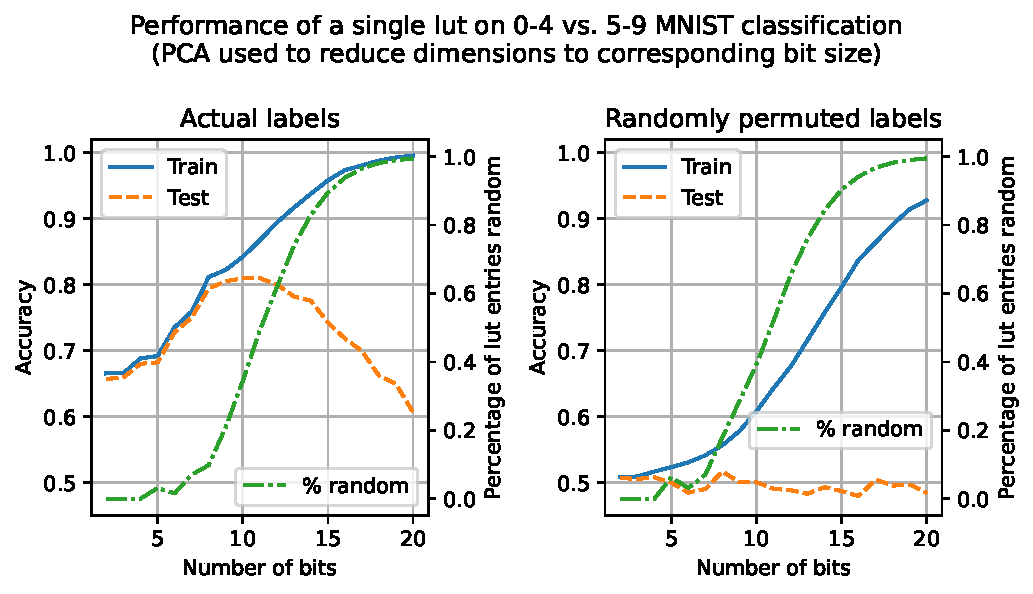
\includegraphics[width=0.99\textwidth,keepaspectratio]{images/single_lut_exp.pdf}
				\end{figure}
\end{frame}

\section{Network of lookup tables ("luts")}


\begin{frame}
	\frametitle{Network}
	\begin{itemize}
		\item As we've seen, a single lut is not very powerful
	\end{itemize}
\end{frame}

\section{How to go from there}

\begin{frame}
\frametitle{How to go from there}
\end{frame}

\section{Recap}
\begin{frame}
	\frametitle{Recap}
	Hello there, this is empty :)
\end{frame}

\begin{frame}
\begin{figure}
\centering
\includegraphics[width=.3\textwidth]{images/schmuser.png}
\end{figure}
\begin{center}
\huge Any Questions?
\end{center}
\end{frame}

\section{References}

\begin{frame}
\frametitle{References lala}
\printbibliography
\end{frame}

\end{document}
